\documentclass[rnd]{mas_proposal}
% \documentclass[thesis]{mas_proposal}

\usepackage[utf8]{inputenc}
\usepackage{amsmath}
\usepackage{amsfonts}
\usepackage{amssymb}
\usepackage{graphicx}

\title{Robot motion planning in dynamic environment: A comparative study}
\author{Dharmin Bakaraniya}
\supervisors{Prof.\ Dr.\ Ervin Prassler\\Dr.\ Cesar Lopez Martinez}

% \thirdpartylogo{path/to/your/image}

\begin{document}

\maketitle

\pagestyle{plain}

\chapter{Introduction}
The topic for this R\&D is motion planning for dynamic environment. 
By solving this problem, we can ensure 
\begin{itemize}
    \item Safe environment for humans and for robots
    \item Cost effective transportation of goods
\end{itemize}
Motion planning in dynamic environment needs to perform the following task
\begin{itemize}
    \item Reach the desired target position
    \item Avoid static and moving obstacle
    \item Consider actuator constraints
    \item Consider geometry of robot
\end{itemize}
It needs to perform these tasks in \textit{fast} and \textit{efficient} manner. 
The \textit{fast} nature of planner dictates that the planning of motion should be at least performed in real time for the robot to react to its environment. 
An approach is \textit{efficient} if the planner
\begin{itemize}
    \item does not collide
    \item takes minimal time to reach goal position
    \item does not require a large amount of sensor data
    \item does not require a lot of computational resources
\end{itemize}

\section{Problem Statement}
\begin{itemize}
    \item Current approaches are not generalised for all types of robot. They work best for circular holonomic robots. Velocity based approaches, which perform very well, are mostly tested on point sized robots.
    \item Some approaches are defined and tested for non-holonomic vehicles, but they either lack in terms of computation speed or they do not guarantee a solution.
    \item Most of the approaches do not even address how the objects needs to be perceived. They do not address how errors from perception and control would influence the planner's efficiency.
    \item This work will provide a comparative study on existing approaches for motion planning in time varying environment.
\end{itemize}

\section{Use case}
\begin{itemize}
    \item This work will consider only indoor environments (hospital, warehouses, university library, etc.) where the mobile robots is supposed to navigate.
    \item Moving obstacles will be humans or other robots.
    \item The model of the environment and the model that humans will follow for their navigation will be provided for each test case.
    \item For example,
        \begin{itemize}
            \item A mobile robot has to pass through a crowed hallway where the humans try to avoid robot.
            \item A mobile robot must cross a large open area containing a reception desk where humans stop if they are going to collide to the robot. Here, the robot must also consider its path such that least amount of humans' time is wasted.
        \end{itemize} 
\end{itemize}
\chapter{Related Work}
\begin{itemize}
    \item All the existing approaches have tested their efficiency on different robots and in different test environment.
    \item As the measuring criterion for each of them is different, it becomes an impossible task to determine a clear winner.
    \item There are several existing survey article:
        \begin{itemize}
            \item Mohanan et al.\cite{mohanan2018a} covers 101 research papers that were published between 1985 and 2016 in the field of motion planning in dynamic environment. 
                They have addressed all the approaches but a comparative analysis of all the approaches with their contributions and deficiencies is left to be desired.
            \item Hoy et al.\cite{hoy2015algorithms} provides a survey for algorithms which provide collision free navigation for robots. 
                This survey is not only detailed but also quite broad as it covers obstacle avoidance algorithm as well. 
                Even though it provides a comparison between main approaches based on numerous criterion, it still does not evaluate these approaches on a standard uniform test.
            \item Keshmiri et al.\cite{keshmiri2009overview} provides a survey specifically for motion planning in dynamic environment. 
                It covers all the approaches presented in research papers published between 1986 and 2008 totalling up to 150 papers. 
                They have provided a comparison on how much contribution has been made in motion planning field based on different approach but regarding the actual approaches itself, only a summary of at most 2\-3 sentences for each approach is provided.
            \item Approaches~\cite{fujimura1991motion} and~\cite{tsubouchi1996motion} are quite dated and does not cover any state of the art approaches in motion planning for dynamic environment.
        \end{itemize}
    \item Existing approaches generally provide critique and deficiencies on their previous works. These are generally helpful but they mostly compare their approach with the existing solutions and only point out the deficiencies that they have addressed. Therefore, though these comparisons are helpful, they might not be completely reliable.
\end{itemize}

\section{Approaches in motion planning for dynamic environment}
\subsection{Velocity based}
\begin{itemize}
    \item \textit{Dynamic window approach}: Fox et al.\cite{fox1997dynamic} proposed the original idea for simply optimizing a function which balances robot's distance from goal, distance from nearest obstacle and current velocity. This approach, despite being robust, simple and fast did not work for dynamic environment. 
        Later, Brock et al.\cite{brock1999high} extended this approach for global path planning and for dynamic environments by combining it with NF1 algorithm. 
        This eradicated the problem of local minima. 
        It has been since extended in~\cite{seder2007dynamic} and~\cite{ogren2005convergent}
    \item \textit{Velocity obstacle (VO)}: Originally developed by Fiorini et al.\cite{fiorini1998motion}, this approach proposes to avoid obstacles by choosing velocity outside \textit{collision cone}.
        This approach unifies the representation for avoiding static and dynamic obstacles.
        This idea has since been transformed to incorporate many scenarios\cite{shiller2010nonlinear}\cite{owen2006a}\cite{owen2005motion}\cite{guy2009clearpath}. 
        For multi robot systems, Van den berg et al.\cite{van2008reciprocal}\cite{van2011reciprocal}\cite{van2006anytime} have extended VO approach.
    \item \textit{ICS based approach}: Inevitable collision states (ICS)\cite{fraichard2004inevitable}\cite{petti2005safe}\cite{martinez2009collision} have proposed a solution to avoid states that has no outcome other than collision. They propose that this states if avoided will ensure that the robot will never collide. They have approached this problem in a mathematical way. They provide a very fast and almost infinite look ahead option\cite{mohanan2018a}.

\end{itemize}

\subsection{Roadmap based}
\begin{itemize}
    \item \textit{Randomized kinodynamic planning}: Hsu et al.\cite{hsu2002randomized} provides an extension of probabilistic roadmap approach by considering kinodynamics of the robot before choosing a motion control.
    \item Van den berg et al.\cite{van2005roadmap} provides an extension on roadmap based motion planning for static and dynamic obstacles.
\end{itemize}

\subsection{Other}
\begin{itemize}
    \item \textit{Nearness diagram}:~\cite{minguez2004nearness} proposes a \textit{divide and conquer} strategy for motion planning in dynamic environment using a geometry based approach for their implementation.
\end{itemize}


\chapter{Project Plan}

\section{Work Packages and milestones}
The bare minimum will include the following packages:
\begin{table}[ht!]
    \centering
    \begin{tabular}{|l|l|}
        \hline
        \textbf{Work packages} & \textbf{Tasks} \\\hline
        Literature review   & Gather literature on motion planning for dynamic environment\\
                            & Define use cases based on general situations of motion planning \\
                            & Create a solid review criteria based on use case\\
                            & Compare different approaches based on review criteria\\
                            & Exclude approaches based on review criteria \\ 
                            & Create annotated bibliography for top 30 approaches\\ 
                            & Create summary of annotated bibliography and add it to report\\\hline
        Identify parameters & Define performance metrics to test approaches \\
        for Experiments     & Identify parameters and assumptions of dynamic environment\\
                            & which will be used for experiments\\
                            & Refine use cases (if needed)\\
                            & Choose top 3 motion planning approaches based on use case\\
                            & Add description of dynamic environment, use cases and \\
                            & performance metrics to report\\\hline
         Experiments        & Implement top 3 motion planning approaches\\ 
                            & Test 3 approaches on use cases and gather results \\ 
                            & Analyse results and provide explanation for it\\
                            & Provide conclusion of experiment\\
                            & Document experiment results, proof and conclusion \\\hline
        Documentation       & Document conclusion and review \\
                            & Refine report for better readability \\\hline 
    
    \end{tabular}
    \caption{Work packages and milestones\label{tab:workpackagesandmilestones}}
\end{table}

\section{Project Schedule}
Please see Figure~\ref{fig:gantt}
\begin{figure}[h!]
    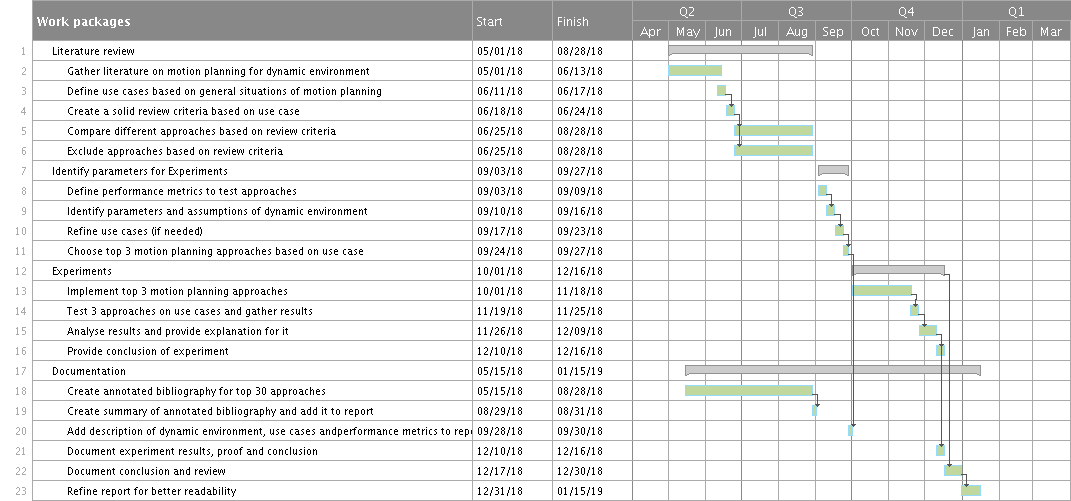
\includegraphics[width=1.0\textwidth]{gantt_chart2.png}
    \caption{Gannt chart for workpackages\label{fig:gantt}}
\end{figure}

\section{Deliverables}
\subsection{Minimum}

\begin{itemize}
    \item Annotated bibliography on top 30 approaches for motion planning in dynamic environment
    \item Description of review criteria, use cases, performance metrics
    \item Comparison of 3 approaches of motion planning in dynamic environment in simulation
    \item Proof of these 3 approaches being best based on experiment results and analysis
    \item R \& D report 
\end{itemize}

\subsection{Expected}
\begin{itemize}
    \item All items in minimum deliverable
    \item Comparison of 3 approaches of motion planning in dynamic environment on actual robot
\end{itemize}

\subsection{Desired}
\begin{itemize}
    \item All items in expected deliverable
    \item Experiment results of 3 approaches on more use cases and complex scenarios
    \item Comparison of an additional algorithm
\end{itemize}

%\nocite{*}

\bibliographystyle{ieeetr} % Use the plainnat bibliography style
\bibliography{../myRef.bib} % Use the bibliography.bib file as the source of references




\end{document}
